\documentclass[12pt, a4paper]{article}

% ── Encoding & Língua ──────────────────────────────────────────────────────
\usepackage[utf8]{inputenc}
\usepackage[T1]{fontenc}
\usepackage[brazil]{babel}

% ── Layout ─────────────────────────────────────────────────────────────────
\usepackage{geometry}
\geometry{
    top    = 3cm,
    bottom = 2.5cm,
    left   = 3cm,
    right  = 2.5cm,
}
\usepackage{setspace}
\onehalfspacing

% ── Matemática ─────────────────────────────────────────────────────────────
\usepackage{amsmath, amssymb, amsthm}
\usepackage{mathtools}

% ── Gráficos & Cores ───────────────────────────────────────────────────────
\usepackage{graphicx}
\usepackage{xcolor}
\definecolor{unicampblue}{RGB}{0, 60, 130}
\definecolor{darkgray}{RGB}{50, 50, 50}

% ── Hyperlinks ─────────────────────────────────────────────────────────────
\usepackage[
    colorlinks = true,
    linkcolor  = unicampblue,
    citecolor  = unicampblue,
    urlcolor   = unicampblue,
]{hyperref}

% ── Referências ────────────────────────────────────────────────────────────
\usepackage[
    backend  = biber,
    style    = numeric,
    sorting  = none,
]{biblatex}
\addbibresource{referencias.bib}

% ── Títulos ────────────────────────────────────────────────────────────────
\usepackage{titlesec}
\titleformat{\section}
    {\color{unicampblue}\large\bfseries}
    {\thesection.}{0.5em}{}[\titlerule]
\titleformat{\subsection}
    {\color{darkgray}\normalsize\bfseries}
    {\thesubsection.}{0.5em}{}

% ── Código ─────────────────────────────────────────────────────────────────
\usepackage{listings}
\lstset{
    basicstyle   = \ttfamily\small,
    keywordstyle = \color{unicampblue}\bfseries,
    commentstyle = \color{gray}\itshape,
    frame        = single,
    breaklines   = true,
}

% ── Cabeçalho / Rodapé ─────────────────────────────────────────────────────
\usepackage{fancyhdr}
\pagestyle{fancy}
\fancyhf{}
\fancyhead[L]{\small\color{gray} MS901 --- Diagnóstico Físico do Resíduo em PINNs}
\fancyhead[R]{\small\color{gray} IMECC / Unicamp}
\fancyfoot[C]{\thepage}
\renewcommand{\headrulewidth}{0.4pt}

% ── Caixas de destaque ─────────────────────────────────────────────────────
\usepackage{tcolorbox}
\tcbuselibrary{skins, breakable}

\newtcolorbox{perguntabox}{
    enhanced,
    colback  = unicampblue!5,
    colframe = unicampblue,
    fonttitle= \bfseries,
    title    = Perguntas de Pesquisa,
    left=6pt, right=6pt,
}

\newtcolorbox{definicaobox}[1]{
    enhanced,
    colback  = gray!8,
    colframe = darkgray,
    fonttitle= \bfseries,
    title    = #1,
    left=6pt, right=6pt,
}

% ── Teoremas ───────────────────────────────────────────────────────────────
\theoremstyle{definition}
\newtheorem{definicao}{Definição}[section]
\newtheorem{proposicao}{Proposição}[section]
\newtheorem{exemplo}{Exemplo}[section]
\newtheorem{observacao}{Observação}[section]

% ── Operadores ─────────────────────────────────────────────────────────────
\newcommand{\loss}{\mathcal{L}}
\newcommand{\pinn}{\hat{u}_\theta}
\newcommand{\N}{\mathcal{N}}
\newcommand{\R}{\mathbb{R}}
\newcommand{\norm}[1]{\left\lVert #1 \right\rVert}
\newcommand{\abs}[1]{\left| #1 \right|}

% ═══════════════════════════════════════════════════════════════════════════
% DOCUMENTO
% ═══════════════════════════════════════════════════════════════════════════

\begin{document}

% ── Capa ───────────────────────────────────────────────────────────────────
\begin{titlepage}
\begin{center}

    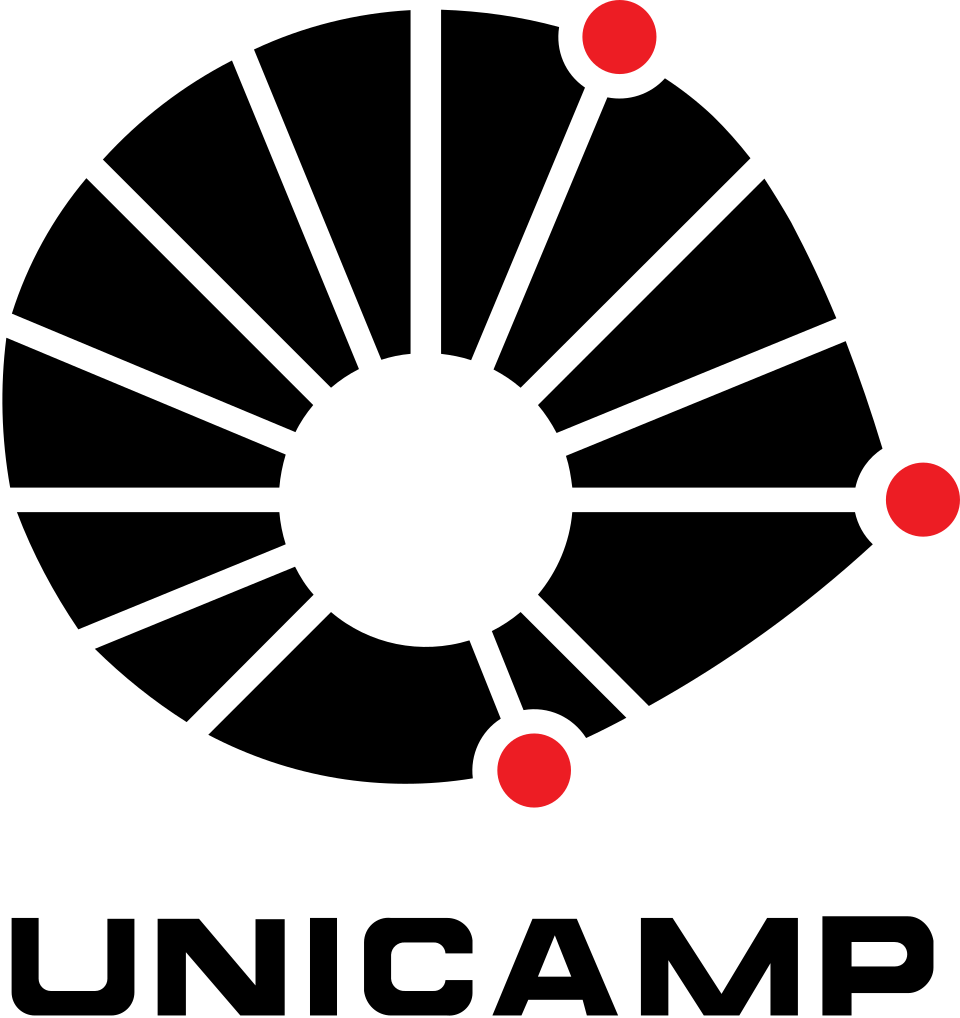
\includegraphics[width=0.35\textwidth]{../../Imagens/UNICAMP_logo.png}

    \vspace{0.6cm}
    {\Large \textbf{Universidade Estadual de Campinas}}\\[0.2cm]
    {\large Instituto de Matemática, Estatística e\\Computação Científica --- IMECC}

    \vspace{1.6cm}
    \rule{\textwidth}{1.2pt}\\[0.3cm]
    {\LARGE \textbf{Diagnóstico Físico do Resíduo em Redes\\[0.15cm]
    Neurais Informadas pela Física (PINNs)}}\\[0.2cm]
    {\large \textit{Uma Análise via Teoria da Equação Modificada}}\\[0.2cm]
    \rule{\textwidth}{1.2pt}

    \vspace{1.6cm}

    \begin{minipage}{0.48\textwidth}
        \begin{flushleft}
            \textbf{Aluno:}\\
            Guilherme Medeiros\\
            RA: 256774
        \end{flushleft}
    \end{minipage}
    \begin{minipage}{0.48\textwidth}
        \begin{flushright}
            \textbf{Disciplina:}\\
            MS901 --- Tópicos Especiais de\\
            Matemática Aplicada (Turma A)\\[0.4cm]
            \textbf{Professores:}\\
            Prof.\ Eduardo Abreu\\
            Prof.\ João Florindo
        \end{flushright}
    \end{minipage}

    \vfill
    {\large IMECC --- Unicamp \\ 1.º Semestre de 2026}

\end{center}
\end{titlepage}

% ── Sumário ────────────────────────────────────────────────────────────────
\tableofcontents
\newpage

% ═══════════════════════════════════════════════════════════════════════════
\section{Introdução}
% ═══════════════════════════════════════════════════════════════════════════

A simulação computacional de fenômenos físicos governados por equações diferenciais parciais
(EDPs) é um dos pilares da Matemática Aplicada moderna. Durante décadas, esse campo foi
dominado por métodos clássicos de discretização --- diferenças finitas, volumes finitos e
elementos finitos --- cujas propriedades de estabilidade, consistência e convergência são
rigorosamente estabelecidas pela Análise Numérica.

Nas últimas décadas, o advento do aprendizado profundo trouxe uma nova família de métodos:
as \textbf{Physics-Informed Neural Networks} (PINNs) \cite{raissi2019}. Em vez de discretizar
o domínio em malhas, as PINNs parametrizam a solução $u(x,t)$ como uma rede neural
$\pinn(x,t; \theta)$ e incorporam a EDP diretamente na função de custo (\textit{loss}):
\begin{equation}
    \loss(\theta) = \underbrace{\frac{1}{N_f}\sum_{i=1}^{N_f}
        \abs{f(x_f^i,\, t_f^i;\,\theta)}^2}_{\text{loss física (resíduo EDP)}}
    \;+\;
    \lambda\underbrace{\frac{1}{N_u}\sum_{j=1}^{N_u}
        \abs{\pinn(x_u^j,t_u^j) - u^j}^2}_{\text{loss de dados (CI/CC)}},
    \label{eq:loss_total}
\end{equation}
onde $f := \partial_t u + \mathcal{N}[u]$ é o resíduo do operador diferencial e
$\{x_u^j, t_u^j, u^j\}$ são os pontos de condição inicial e de contorno.

A beleza da abordagem está na sua generalidade: não há malha, não há restrições de
dimensionalidade impostas pela discretização, e a rede pode, em princípio, aproximar
soluções de problemas de alta dimensão onde os métodos clássicos sucumbem à
\textit{maldição da dimensionalidade}.

Entretanto, essa flexibilidade vem com um custo epistemológico relevante: ao minimizar
$\loss(\theta)$, raramente se atinge o resíduo nulo. Isso significa que a rede não está
resolvendo a EDP original, mas sim uma \textbf{equação perturbada}:
\begin{equation}
    \partial_t \pinn + \mathcal{N}[\pinn] = r(x, t),
    \label{eq:edp_perturbada}
\end{equation}
onde $r(x,t)$ é o campo de resíduo da rede treinada. A pergunta central deste trabalho
é precisamente:

\begin{perguntabox}
\textit{O que o resíduo residual $r(x,t)$ de uma PINN está fazendo com a física que
ela deveria resolver? Ele age como uma perturbação difusiva, introduzindo viscosidade
artificial? Ou age como uma perturbação dispersiva, gerando oscilações espúrias?
E como a escolha da arquitetura da rede influencia essa perturbação?}
\end{perguntabox}

A resposta a essas perguntas é fornecida pela \textbf{Teoria da Equação Modificada},
um instrumento clássico de Análise Numérica que, neste trabalho, é transplantado
para o contexto das redes neurais.

% ═══════════════════════════════════════════════════════════════════════════
\section{Motivação e Contexto}
% ═══════════════════════════════════════════════════════════════════════════

\subsection{O Problema da Análise do Erro em PINNs}

A convergência dos métodos numéricos clássicos é garantida pelo Teorema de
Lax-Richtmyer: um método consistente e estável é necessariamente convergente.
Esse teorema conecta três conceitos bem definidos --- consistência (o esquema
aproxima bem a EDP), estabilidade (o erro não cresce sem controle) e convergência
(a solução numérica se aproxima da solução exata quando o passo tende a zero).

Para PINNs, esse quadro é mais nebuloso. A loss $\loss(\theta)$ mede o resíduo
em pontos de colocação, mas não há uma teoria geral que conecte o valor da loss
à distância $\norm{\pinn - u_{\text{exata}}}$ de forma tão precisa quanto nos métodos
clássicos. Pior: uma loss pequena pode coexistir com erros grandes em regiões do
domínio mal cobertas pelos pontos de colocação.

\subsection{A Teoria da Equação Modificada como Ferramenta de Auditoria}

A Teoria da Equação Modificada, introduzida por Hirt \cite{hirt1968} no contexto de
diferenças finitas, oferece uma resposta elegante a uma pergunta análoga: \textit{qual
equação um esquema numérico está efetivamente resolvendo?}

A ideia central é expandir os termos do esquema numérico em série de Taylor ao redor
do ponto exato e identificar os termos de erro dominantes. Para o esquema de
Lax-Friedrichs aplicado à advecção linear $u_t + a\,u_x = 0$, por exemplo,
a equação modificada é:
\begin{equation}
    u_t + a\,u_x = \underbrace{\nu_{\mathrm{LF}}\, u_{xx}}_{\text{difusão artificial}}
    + \mathcal{O}(\Delta x^2),
    \qquad
    \nu_{\mathrm{LF}} = \frac{\Delta x}{2}\bigl(1 - \mathrm{CFL}\bigr),
    \label{eq:eq_modificada_lf}
\end{equation}
revelando que o esquema é difusivo de primeira ordem.

A proposição central deste trabalho é a seguinte:

\begin{definicaobox}{Equação Modificada Neural}
Dado uma PINN treinada $\pinn$ com resíduo $r(x,t) \neq 0$, definimos a
\textbf{equação modificada neural} como
\begin{equation}
    \partial_t \pinn + \mathcal{N}[\pinn]
    \;=\;
    \nu_{\mathrm{num}}\, \partial_{xx}\pinn
    \;+\;
    \beta_{\mathrm{num}}\, \partial_{xxx}\pinn
    \;+\;
    \mathcal{O}(\text{termos de ordem superior}),
    \label{eq:eq_modificada_neural}
\end{equation}
onde $\nu_{\mathrm{num}} \geq 0$ é a \textbf{viscosidade numérica neural} e
$\beta_{\mathrm{num}}$ é o coeficiente de \textbf{dispersão numérica neural}.
O resíduo age como uma perturbação da EDP original: se $\nu_{\mathrm{num}}$
domina, a rede suaviza a solução (difusão); se $\beta_{\mathrm{num}}$ domina,
a rede introduz oscilações (dispersão).
\end{definicaobox}

\subsection{Por que isso importa?}

O diagnóstico da equação modificada neural tem implicações práticas diretas:

\begin{enumerate}
    \item \textbf{Estabilidade física:} um $\nu_{\mathrm{num}} > 0$ grande indica que
    a rede está ``amortecendo'' a solução, potencialmente suavizando descontinuidades
    como choques --- exatamente o oposto do comportamento desejado em leis de conservação
    hiperbólicas.

    \item \textbf{Escolha de arquitetura:} se $\nu_{\mathrm{num}}$ depende da
    função de ativação, da profundidade ou da largura da rede, então a escolha
    arquitetural tem interpretação física, não apenas empírica.

    \item \textbf{Conexão AN--SciML:} o mesmo coeficiente $\nu_{\mathrm{num}}$
    calculado para métodos clássicos (Equação~\ref{eq:eq_modificada_lf}) pode ser
    calculado para PINNs, permitindo uma comparação direta e fundamentada.
\end{enumerate}

% ═══════════════════════════════════════════════════════════════════════════
\section{Estrutura do Projeto}
% ═══════════════════════════════════════════════════════════════════════════

O projeto está organizado em torno de dois modelos-problema, de complexidade crescente,
aplicados à mesma metodologia de diagnóstico.

\subsection{Modelo I: Equação de Advecção Linear}

O ponto de partida é a equação de advecção linear,
\begin{equation}
    u_t + a\,u_x = 0, \quad x \in [x_{\min}, x_{\max}],\quad t \in [0, T],
    \label{eq:adveccao}
\end{equation}
com velocidade de advecção constante $a > 0$ e condição inicial $u(x, 0) = u_0(x)$.

Esta equação tem solução exata via método das características, $u(x,t) = u_0(x - at)$,
o que permite medir o erro exato da PINN e calibrar o diagnóstico. Adicionalmente, a
estimativa de energia de Gronwall,
\begin{equation}
    \int u^2(x,t)\,dx \;\leq\; e^{\norm{a}_{C^1} \cdot t} \int u_0^2(x)\,dx,
    \label{eq:gronwall}
\end{equation}
fornece uma cota física que a solução da PINN deve respeitar.

\subsection{Modelo II: Equação de Burgers Invíscida}

O segundo modelo é a equação de Burgers invíscida,
\begin{equation}
    u_t + \left(\frac{u^2}{2}\right)_x = 0, \quad x \in \Omega,\quad t \in [0, T],
    \label{eq:burgers}
\end{equation}
com dados iniciais de Riemann (choque ou rarefação). Este é o teste de fogo: a
solução desenvolve uma descontinuidade (choque) em tempo finito, e o comportamento
do resíduo próximo ao choque revela se a PINN introduz viscosidade artificial
suficiente para estabilizar a solução ou se gera oscilações dispersivas.

A solução exata do problema de Riemann para choque é
$u(x,t) = u_L \cdot \mathbf{1}_{x < s t} + u_R \cdot \mathbf{1}_{x \geq st}$,
onde $s = (u_L + u_R)/2$ é a velocidade do choque dada pela condição de
Rankine-Hugoniot.

\subsection{Metodologia de Diagnóstico}

Para ambos os modelos, o diagnóstico segue o mesmo protocolo:

\begin{enumerate}
    \item \textbf{Treinamento da PINN} com a arquitetura em análise (minimização
    da Equação~\ref{eq:loss_total}).

    \item \textbf{Cálculo do campo de resíduo} $r(x, t_0)$ em instantes fixados
    $t_0 \in (0, T]$, usando diferenciação automática.

    \item \textbf{Análise espectral via FFT}: transformada de Fourier discreta do
    resíduo $\hat{R}(k)$ e da solução $\hat{U}(k)$.

    \item \textbf{Estimativa de $\nu_{\mathrm{num}}$}: se o resíduo é dominado por
    difusão, então $\hat{R}(k) \approx \nu_{\mathrm{num}} k^2 \hat{U}(k)$, logo
    \begin{equation}
        \nu_{\mathrm{num}} \approx \operatorname{mediana}
        \left\{\frac{|\hat{R}(k)|}{k^2 |\hat{U}(k)|}\right\}_{k > 0}.
        \label{eq:nu_num}
    \end{equation}

    \item \textbf{Classificação}: comparação da energia espectral em baixas e altas
    frequências para determinar se o erro é predominantemente difusivo ou dispersivo.
\end{enumerate}

% ═══════════════════════════════════════════════════════════════════════════
\section{Perguntas de Pesquisa}
% ═══════════════════════════════════════════════════════════════════════════

O projeto busca responder às seguintes perguntas, em ordem crescente de profundidade:

\begin{enumerate}

    \item \textbf{[Diagnóstico base]} Para uma PINN treinada na equação de advecção
    linear com condição inicial suave ($u_0 = \sin(\pi x)$), o resíduo residual
    é classificado como difusivo ou dispersivo? Qual é a ordem de grandeza de
    $\nu_{\mathrm{num}}$?

    \item \textbf{[Sensibilidade arquitetural]} Como $\nu_{\mathrm{num}}$ varia
    com a escolha de: (a) função de ativação (\texttt{tanh}, \texttt{sin},
    \texttt{relu}, \texttt{swish}); (b) número de neurônios por camada;
    (c) profundidade da rede; (d) número de pontos de colocação $N_f$?

    \item \textbf{[Comparação AN--SciML]} O $\nu_{\mathrm{num}}$ estimado para a
    PINN é comparável ao $\nu_{\mathrm{LF}}$ do método de Lax-Friedrichs com o
    mesmo custo computacional? A PINN consegue atingir viscosidade artificial menor
    do que métodos clássicos de primeira ordem?

    \item \textbf{[Robustez em dados descontínuos]} O diagnóstico se mantém coerente
    quando a condição inicial é descontínua (dado de Riemann)? O resíduo se concentra
    na região do choque? O comportamento muda para a equação de Burgers?

    \item \textbf{[Relação loss--erro físico]} Existe correlação entre o valor
    escalar da loss $\loss(\theta)$ e a viscosidade numérica $\nu_{\mathrm{num}}$?
    Uma loss menor implica necessariamente menor perturbação da física?

\end{enumerate}

% ═══════════════════════════════════════════════════════════════════════════
% REFERÊNCIAS
% ═══════════════════════════════════════════════════════════════════════════

\newpage
\printbibliography[title={Referências}]

\end{document}
